\documentclass[a4paper,11pt,abstracton]{scrartcl}

\usepackage[margin=3cm]{geometry}
\usepackage{graphicx}
\usepackage[UKenglish]{babel}
\usepackage{csquotes}
\usepackage[style=numeric,citestyle=numeric,backend=biber,sorting=none,doi=false,url=false]{biblatex}
\usepackage{float}
\usepackage[export]{adjustbox}
\usepackage[T1]{fontenc}
\usepackage{lmodern}
\usepackage[textsize=tiny]{todonotes}
\usepackage[labelsep=period,font=small,labelfont=bf,format=plain]{caption}
\captionsetup[table]{
  position=above,
  belowskip=10pt,
  aboveskip=0pt,
}
\usepackage[group-separator={,}]{siunitx}
\usepackage{booktabs}
\usepackage{pdflscape}
\usepackage{tablefootnote}
\usepackage{authblk}
\usepackage{threeparttable}
\usepackage{afterpage}
\usepackage{lineno}
\linenumbers
\usepackage{setspace}
\doublespacing


\addbibresource{refs.bib}


\title{
The genetic architecture of target-site resistance to pyrethroid insecticides in the African malaria vectors \emph{Anopheles gambiae} and \emph{Anopheles coluzzii}
}


\date{Work in progress}


\author[1]{Chris S. Clarkson}
\author[2,1]{Alistair Miles}
\author[2]{Nicholas J. Harding}
\author{@@TODO}
\author[1,2]{Dominic Kwiatkowski}
\author[3,1]{Martin Donnelly}
\author[4]{The \emph{Anopheles gambiae} 1000 Genomes Consortium}
\affil[1]{Sanger @@TODO}
\affil[2]{Oxford @@TODO}
\affil[3]{Liverpool @@TODO}
\affil[4]{MalariaGEN @@TODO}


\begin{document}


\maketitle


\begin{abstract}


%%
Resistance to pyrethroid insecticides is a major concern for malaria vector control, because these are the only compounds approved for use in insecticide-treated bed-nets (ITNs) and are also widely used for indoor residual spraying (IRS). 
%
Pyrethroids target the voltage-gated sodium channel (VGSC), an essential component of the mosquito nervous system, but mutations in the \emph{Vgsc} gene can disrupt the activity of these insecticides, inducing a ``knock-down resistance'' phenotype. 
%
Here we use Illumina whole-genome sequence data from phase 1 of the \emph{Anopheles gambiae} 1000 Genomes Project (Ag1000G) to provide a comprehensive account of genetic variation at the \emph{Vgsc} locus in mosquito populations from 8 African countries.
%
In addition to three known resistance variants that alter the protein-coding sequence of the \emph{Vgsc} gene, we describe 19 previously unknown non-synonymous variants at appreciable frequency in one or more populations.
%
For each variant we predict a resistance phenotype based on genetic evidence for recent selection, patterns of linkage between variants, the position of the variant within the protein structure, and experimental evidence from other species.
%
We use analyses of haplotype structure to refine our understanding of the origins and spread of these resistance variants between species and geographical locations.
%
These analyses identify 10 distinct lineages, each of which carries one or more resistance alleles and appears to be undergoing rapid and recent expansion in one or more populations.
%
The most successful and widespread resistance lineage (F1) originates in West Africa and has subsequently spread to countries in Central and Southern Africa.
%
We also reconstruct a putative ancestral haplotype for each lineage, and analyse patterns of recombination to show that lineages are unrelated and thus represent independent outbreaks of resistance.
%
Our data demonstrate that the molecular basis of pyrethroid resistance in African malaria vectors is more complex than previously appreciated, and provide a foundation for the development of new genetic tools to inform insecticide resistance management and track the further spread of resistance.
%%

\end{abstract}


\section*{Introduction}


%% Paragraph 1: The relevance of insecticide resistance to malaria. Start broad, explain why insecticide resistance is relevant to malaria control. Briefly review some of the evidence of the actual and potential impact of insecticide resistance on intervention efficacy and disease prevalence.
%
An estimated 663 million cases of malaria were averted in Africa between 2000 and 2015 due to public health interventions, of which 68\% were prevented by insecticide-treated bed-nets (ITNs) and @@N\% through indoor residual spraying of insecticides (IRS).
%
However, over this same period, insecticide resistance has become increasingly prevalent in malaria vector populations.
%
Four chemical classes of insecticides -- organophosphates, carbamates, pyrethroids and organochlorines -- are licensed for use in public health, but only pyrethroids are approved by the World Health Organisation (WHO) for use in ITNs.
%
Pyrethroids are also commonly used for IRS and in agriculture, and mosquito populations are under pressure to evolve molecular mechanisms of pyrethroid resistance.
%
There is evidence that pyrethroid resistance has a direct impact on the effectiveness of ITNs and IRS, although assessing the impact on disease prevalence is difficult and has been hampered by the fact that pyrethroid resistance is now so pervasive that it is nearly impossible to find fully susceptible mosquito populations to serve as controls.
%
Nevertheless, the position of the WHO remains that insecticide resistance poses a grave threat to the future of malaria control in Africa (@@REF GPIRM).
%
Improvements are needed in our ability to monitor resistance, and gaps must be filled in our knowledge of the molecular mechanisms of resistance.
%%


%% Paragraph 2: Introduce VGSC and concept of target-site resistance. What is known about target-site resistance in An. gambiae.
%
The voltage-gated sodium channel (VGSC) is the physiological target of pyrethroids and of the organochlorine DDT.
%
The VGSC protein is integral to the insect nervous system, involved in the transmission of nerve impulses.
%
Both pyrethroids and DDT have a similar mode of action, binding to sites within the protein channel and preventing normal nerve function, causing paralysis (``knock-down'') and then death.
%
However, amino acid substitutions at key positions within the channel can alter the interaction between the channel and the insecticide molecule, and thereby substantially increase the dosage of insecticide required for knock-down.
%
If this tolerance exceeds the dosage present in ITNs or on indoor surfaces following IRS, these interventions may be rendered ineffective.
%
In the African malaria vectors \emph{Anopheles gambiae} and \emph{Anopheles coluzzii}, three substitutions have been found in natural populations and shown to cause pyrethroid and DDT resistance.
%
Two of these substitutions occur in codon 995\footnotemark, with the Leucine $\rightarrow$ Phenylalanine (\texttt{L995F}) substitution prevalent in West and Central Africa, and the Leucine $\rightarrow$ Serine (\texttt{L995S}) substitution found in Central and East Africa.
%
\footnotetext{Codon numbering is given here relative to transcript @@TODO as defined in the AgamP4.@@N gene annotations. A mapping of codon numbers from @@TRANSCRIPT to \emph{Musca domestica} @@TRANSCRIPT is given in Table \ref{table:variants_missense}.}
%
A third variant \texttt{N1570Y} has been found in association with \texttt{L995F} in Central Africa and shown to increase resistance above \texttt{L995F} alone.
%%


%% Paragraph 3: What is known about VGSC and target-site resistance in other insects. Highlight work on other species that shows there could be many other variants that potentially cause resistance. Studies in An. gambiae have been limited to date. So there could be more to discover (i.e., anticipating our new discoveries).
%
Target-site resistance to pyrethroids and DDT has also been studied in a range of other insect species, including disease vectors as well as domestic and crop pests.
%
Because of its essential function, the VGSC protein is highly conserved across insect species, and knowledge gained from one species is relevant to another.
%
Many resistance-associated variants have been described in these other species, and thus there are many possible amino acid substitutions that could induce a resistance phenotype in malaria vectors, other than the known variants in codons 995 and 1570.
%
Some of these variants are within the trans-membrane channel, and thus may directly interact with insecticide molecules.
%
However, functional studies have also demonstrated that variants within internal linker domains can substantially enhance the the level of resistance, when present in combination with channel modifications.
%
Most previous studies of \emph{An. gambiae} and/or \emph{An. coluzzii} have performed targeted sequencing of small regions within the gene, and there has been no comprehensive survey of variation across the entire gene in multiple populations.
%%


%% Paragraph 4: Origins and spread of resistance. Review what is and isn't known about multiple origins and spread of VGSC resistance in An. gambiae. Explain the idea of origins and spread. Introduce why it's important/useful to know more about origins and spread.
%
Insecticide resistance monitoring in malaria vector populations now often incorporates some form of genetic assay to detect the allele present at \emph{Vgsc} codon 995.
%
Both alleles are present at high frequency in multiple geographical locations, and the \texttt{L995F} allele is present in both \emph{An. gambiae} and \emph{An. coluzzii}.
%
The extent of mosquito migration remains an open question, however mosquitoes do travel between different locations and have the potential to spread resistance alleles from one population to another (adaptive gene flow).
%
Hybridization between mosquito species also occurs and has the potential to transfer resistance alleles between species (adaptive introgression).
%
Studies in West African have shown that the \texttt{L995F} allele has been transferred from \emph{An. gambiae} into \emph{An. coluzzii} populations.
%
A resistance allele may also arise independently in multiple populations, either because of multiple mutational events occurring after insecticides are introduced (selection on new mutations), or because resistance alleles were already present at low frequency in mosquito populations prior to insecticide use (selection on standing variation).
%
Previous studies have found evidence that the \texttt{L995F} allele occurs on several different genetic backgrounds, suggesting multiple origins of resistance.
%
However, these studies have used information from only a small region of the gene, and have limited resolution to make inferences about geographical origins or history of spread.
%
Better information about the origins and spread of resistance could improve insecticide resistance monitoring and inform strategies for insecticide resistance management.
%%


%% Paragraph 5: Segue into results. What we cover in this paper. Explain relationship to previously reported analyses in Ag1000G phase 1 paper.
%
Here we provide a detailed and comprehensive account of genetic variation within the \emph{Vgsc} gene using data from phase 1 of the \emph{Anopheles gambiae} 1000 Genomes Project (Ag1000G).
%
We use genotype and haplotype data derived from whole-genome Illumina sequencing of 765 individual mosquitoes collected from natural populations in 8 African countries to survey genetic diversity and study the evolutionary and demographic history of insecticide resistance at the \emph{Vgsc} locus.
%
Our results reveal an unexpected diversity of molecular mechanisms of resistance, and shed new light on the evolutionary processes underlying the rapid increase in the prevalence of resistance across multiple mosquito populations.
%%


%%%%%%%%%%%%%%%%%%%%%%%%%%%%%%%%%%%%%%%%%%%%%%%%%%%%%%%%%%%%%%%%%%%%%%%%%%%%%%%
%%%%%%%%%%%%%%%%%%%%%%%%%%%%%%%%%%%%%%%%%%%%%%%%%%%%%%%%%%%%%%%%%%%%%%%%%%%%%%%
\section*{Results}


%%%%%%%%%%%%%%%%%%%%%%%%%%%%%%%%%%%%%%%%%%%%%%%%%%%%%%%%%%%%%%%%%%%%%%%%%%%%%%%
\subsection*{Functional variation}


%% Paragraph 1 - Discovery of potentially functional SNPs. I.e., how we came to table 1. What we found there. Reference Ag1000G phase 1 paper, how this paper and results related.
%
To identify single nucleotide polymorphisms (SNPs) with a potentially functional role in pyrethroid resistance, we extracted SNPs from the Ag1000G phase 1 data resource that alter the amino acid sequence of the VGSC protein, and computed their allele frequencies among 9 populations defined by species and country of origin.
%
SNPs that confer resistance are expected to increase in frequency under selective pressure, and we refined the list of potentially functional SNPs to retain only those at an appreciable frequency (>5\%) in one or more populations (Table \ref{table:variants_missense}).
%
The resulting list comprises 20 SNPs, including the known \texttt{L995F}, \texttt{L995S} and \texttt{N1570Y} variants, and a further 17 SNPs not previously described in these species.
%
We reported 15 of these novel SNPs in our initial analysis of the Ag1000G phase 1 data (@@REF Ag1000G), and we extend the analyses here to incorporate two tri-allelic SNPs affecting codons 402 and 410.
%%


%% Table 1 - Functional SNPs.
%
\afterpage{%
%\clearpage
% N.B., for some reason using \newgeometry causes page number to get dropped from the subsequent page, so disable for now - not needed if using \footnotesize.
%\newgeometry{margin=2cm}
\begin{landscape}
\thispagestyle{empty}
\begin{table}[h]
  \footnotesize
  \centering
  \begin{threeparttable}

  \caption{
%
\textbf{Non-synonymous nucleotide variation in the voltage-gated sodium channel gene}. 
%
AO=Angola; BF=Burkina Faso; GN=Guinea; CM=Cameroon; GA=Gabon; UG=Uganda; KE=Kenya; GW=Guinea-Bissau; \textit{Ac}=\textit{An. coluzzii}; \textit{Ag}=\textit{An. gambiae}.
%
All variants are at 5\% frequency or above in one or more of the 9 Ag1000G phase 1 populations, with the exception of \texttt{2,400,071 G>T} which is only found in the CM\emph{Ag} population at 0.4\% frequency but is included because another mutation (\texttt{2,400,071 G>A}) is found at the same position causing the same amino acid substitution (\texttt{M490I}); and \texttt{2,431,019 T>C} (\texttt{F1920S}) which is at 4\% frequency in GA\emph{Ag} but also found in CM\emph{Ag} and linked to \texttt{L995F}. 
}

  
\begin{tabular}{lllrrrrrrrrrrr}
\toprule
\multicolumn{3}{c}{Mutation} &
\multicolumn{9}{c}{Population allele frequency (\%)} &
\multicolumn{2}{c}{LD ($D'$)} \\
\cmidrule(r){1-3}
\cmidrule(r){4-12}
\cmidrule(r){13-14}
Position\tablefootnote{Position relative to AgamP3 reference sequence, chromosome arm 2L.} & 
\emph{Ag}\tablefootnote{Codon numbering according to transcript \texttt{AGAP004707-RA} in geneset AgamP4.4.} & 
\emph{Md}\tablefootnote{Codon numbering according to \emph{Musca domestica Vgsc} EMBL accession X96668 \cite{williamson1996}.} & 
AO\emph{Ac} & 
BF\emph{Ac} & 
GN\emph{Ag} & 
BF\emph{Ag} & 
CM\emph{Ag} & 
GA\emph{Ag} & 
UG\emph{Ag} & 
KE & 
GW & 
\texttt{L995S} & 
\texttt{L995F} \\
\midrule

\texttt{2,390,177 G>A} & \texttt{R254K} & \texttt{R261} & 0 & 0 & 0 & 0 & 32 & 21 & 0 & 0 & 0 & -0.98 & 0.96 \\

\texttt{2,391,228 G>C} & \texttt{V402L} & \texttt{V410} & 0 & 7 & 0 & 0 & 0 & 0 & 0 & 0 & 0 & -1 & -0.41 \\

\texttt{2,391,228 G>T} & \texttt{V402L} & \texttt{V410} & 0 & 7 & 0 & 0 & 0 & 0 & 0 & 0 & 0 & -1 & 0.10 \\

\texttt{2,399,997 G>C} & \texttt{D466H} & \texttt{-} & 0 & 0 & 0 & 0 & 7 & 0 & 0 & 0 & 0 & -1 & 1 \\

\texttt{2,400,071 G>A} & \texttt{M490I} & \texttt{M508} & 0 & 0 & 0 & 0 & 0 & 0 & 0 & 18 & 0 & -0.33 & -1 \\

\texttt{2,400,071 G>T} & \texttt{M490I} & \texttt{M508} & 0 & 0 & 0 & 0 & 0 & 0 & 0 & 0 & 0 & -1 & -0.01 \\

\texttt{2,416,980 C>T} & \texttt{T791M} & \texttt{T810} & 0 & 1 & 13 & 14 & 0 & 0 & 0 & 0 & 0 & -1 & 1 \\

\texttt{2,422,651 T>C} & \texttt{L995S} & \texttt{L1014} & 0 & 0 & 0 & 0 & 15 & 64 & 100 & 76 & 0 & 1 & -1 \\

\texttt{2,422,652 A>T} & \texttt{L995F} & \texttt{L1014} & 86 & 85 & 100 & 100 & 53 & 36 & 0 & 0 & 0 & -1 & 1 \\

\texttt{2,424,384 C>T} & \texttt{A1125V} & \texttt{K1133} & 9 & 0 & 0 & 0 & 0 & 0 & 0 & 0 & 0 & -1 & -1 \\

\texttt{2,425,077 G>A} & \texttt{V1254I} & \texttt{I1262} & 0 & 0 & 0 & 0 & 0 & 0 & 0 & 0 & 5 & -1 & -1 \\

\texttt{2,429,617 T>C} & \texttt{I1527T} & \texttt{I1532} & 0 & 14 & 0 & 0 & 0 & 0 & 0 & 0 & 0 & -1 & -1 \\

\texttt{2,429,745 A>T*} & \texttt{N1570Y} & \texttt{N1575} & 0 & 26 & 10 & 22 & 6 & 0 & 0 & 0 & 0 & -1 & 0.98 \\

\texttt{2,429,897 A>G} & \texttt{E1597G} & \texttt{E1602} & 0 & 0 & 6 & 4 & 0 & 0 & 0 & 0 & 0 & -1 & 1 \\

\texttt{2,429,915 A>C} & \texttt{K1603T} & \texttt{K1608} & 0 & 5 & 0 & 0 & 0 & 0 & 0 & 0 & 0 & -1 & 1 \\

\texttt{2,430,424 G>T} & \texttt{A1746S} & \texttt{A1751} & 0 & 0 & 11 & 13 & 0 & 0 & 0 & 0 & 0 & -1 & 1 \\

\texttt{2,430,817 G>A} & \texttt{V1853I} & \texttt{V1858} & 0 & 0 & 8 & 5 & 0 & 0 & 0 & 0 & 0 & -1 & 1 \\

\texttt{2,430,863 T>C} & \texttt{I1868T} & \texttt{I1873} & 0 & 0 & 18 & 25 & 0 & 0 & 0 & 0 & 0 & -1 & 1 \\

\texttt{2,430,880 C>T} & \texttt{P1874S} & \texttt{P1879} & 0 & 21 & 0 & 0 & 0 & 0 & 0 & 0 & 0 & -1 & 1 \\

\texttt{2,430,881 C>T} & \texttt{P1874L} & \texttt{P1879} & 0 & 7 & 45 & 26 & 0 & 0 & 0 & 0 & 0 & -1 & 1 \\

\texttt{2,431,061 C>T} & \texttt{A1934V} & \texttt{A1939} & 0 & 12 & 0 & 0 & 0 & 0 & 0 & 0 & 0 & -1 & 1 \\

\texttt{2,431,079 T>C} & \texttt{I1940T} & \texttt{I1945} & 0 & 4 & 0 & 0 & 7 & 0 & 0 & 0 & 0 & -1 & 1 \\

\bottomrule
\end{tabular}

  
  \begin{tablenotes}
    \footnotesize
    
    \item[1] Position relative to the AgamP3 reference sequence, chromosome arm 2L. Variants marked with an asterisk (*) failed conservative variant filters applied genome-wide in the Ag1000G phase 1 AR3 callset, but appeared sound on manual inspection of read alignments.
    
    \item[2] Codon numbering according to \emph{Anopheles gambiae} transcript AGAP004707-RA in geneset AgamP4.4.
    
    \item[3] Codon numbering according to \emph{Musca domestica} EMBL accession X96668 \cite{williamson1996}.
    
    \item[4] Position of the variant within the protein. \texttt{IN}=internal domain; \texttt{TM}=trans-membrane domain. The protein contains four homologous repeats (I-IV), each having six transmembrane segments (1-6). Codes in parentheses identify the specific domain, e.g., ``\texttt{I.S4}'' refers to trans-membrane segment 4 in repeat I, and ``\texttt{IS4--IS5}'' refers to the linker segment between \texttt{I.S4} and \texttt{I.S5}.
    
    \item[5] Phenotype predictions are based on population genetic evidence and have not been confirmed experimentally.
    
  \end{tablenotes}
  
  \end{threeparttable}
  
  \label{table:variants_missense}
  
\end{table}
\end{landscape}
%\restoregeometry
} % end afterpage
%% end Table 1


%% Paragraph 2 - Findings for 995 variants. Frequencies. Cite evidence for selection. Clearly main drivers of resistance. Hardy-Weinberg results.
%
The two alleles in codon 995 are clearly the main drivers of resistance at this locus.
%
The \texttt{L995F} allele at high frequency in populations of both species from West, Central and Southern Africa, and the \texttt{L995S} allele at high frequency among \textit{An. gambiae} populations from Central and East Africa (Table \ref{table:variants_missense}; @@REF Ag1000G).
%
All haplotypes carrying L995F or L995S have evidence for strong recent positive selection (@@REF Ag1000G).
%
Both alleles were present in populations sampled from Cameroon and Gabon, including some individuals with a hybrid \texttt{L995F/S} genotype. Within these populations, the \texttt{L995F} and \texttt{L995S} alleles were (@@TODO were not?) in Hardy-Weinberg equilibrium (P=@@), thus there does not (@@does?) appear to be selection against hybrids.
%%


%% Paragraph 3 - Results for I1527T and V402L.
%
The \texttt{I1527T} allele is present in \textit{An. coluzzii} from Burkina Faso at 14\% frequency, and there is evidence that haplotypes carrying this allele have been positively selected (@@REF Ag1000G).
%
Codon 1527 occurs within trans-membrane domain segment \texttt{III.S6}, immediately adjacent to a second predicted binding pocket for pyrethroid molecules, thus it is plausible that \texttt{I1527T} could alter insecticide binding (@@REF Dong).
%
We also found that the two variant alleles affecting codon 402, both of which induce a \texttt{V402L} substitution, were in strong linkage with \texttt{I1527T} (D'>@@N; Figure @@LD), and almost all haplotypes carrying \texttt{I1527T} also carried a \texttt{V402L} substitution.
%
The most parsimonious explanation for this pattern of linkage is that the \texttt{I1527T} mutation occurred first, and mutations in codon 402 subsequently arose on this genetic background.
%
Codon 402 also occurs within a trans-membrane segment (\texttt{I.S6}), and the \texttt{V402L} substitution has by itself been shown experimentally to increase pyrethroid resistance in @@species and \textit{Xenopus} oocytes (@@REFs).
%
However, because \texttt{V402L} appears secondary to \texttt{I1527T} in our cohort, we classify \texttt{I1527T} as a putative resistance driver and \texttt{V402L} as a putative enhancer.
%
Because of the limited geographical distribution of these alleles, we hypothesize that the \texttt{I1527T+V402L} combination represents a pyrethroid resistance allele that arose in West African \textit{An. coluzzii} populations; however, the \texttt{L995F} allele is at higher frequency (85\%) in our Burkina Faso \textit{An. coluzzii} population, and is known to be increasing in frequency (@@REFs), therefore \texttt{L995F} may provide a stronger resistance phenotype and is replacing \texttt{I1527T+V402L} in these populations.
%%


%% Figure - Pairwise LD.
%
\begin{figure}[!t]

  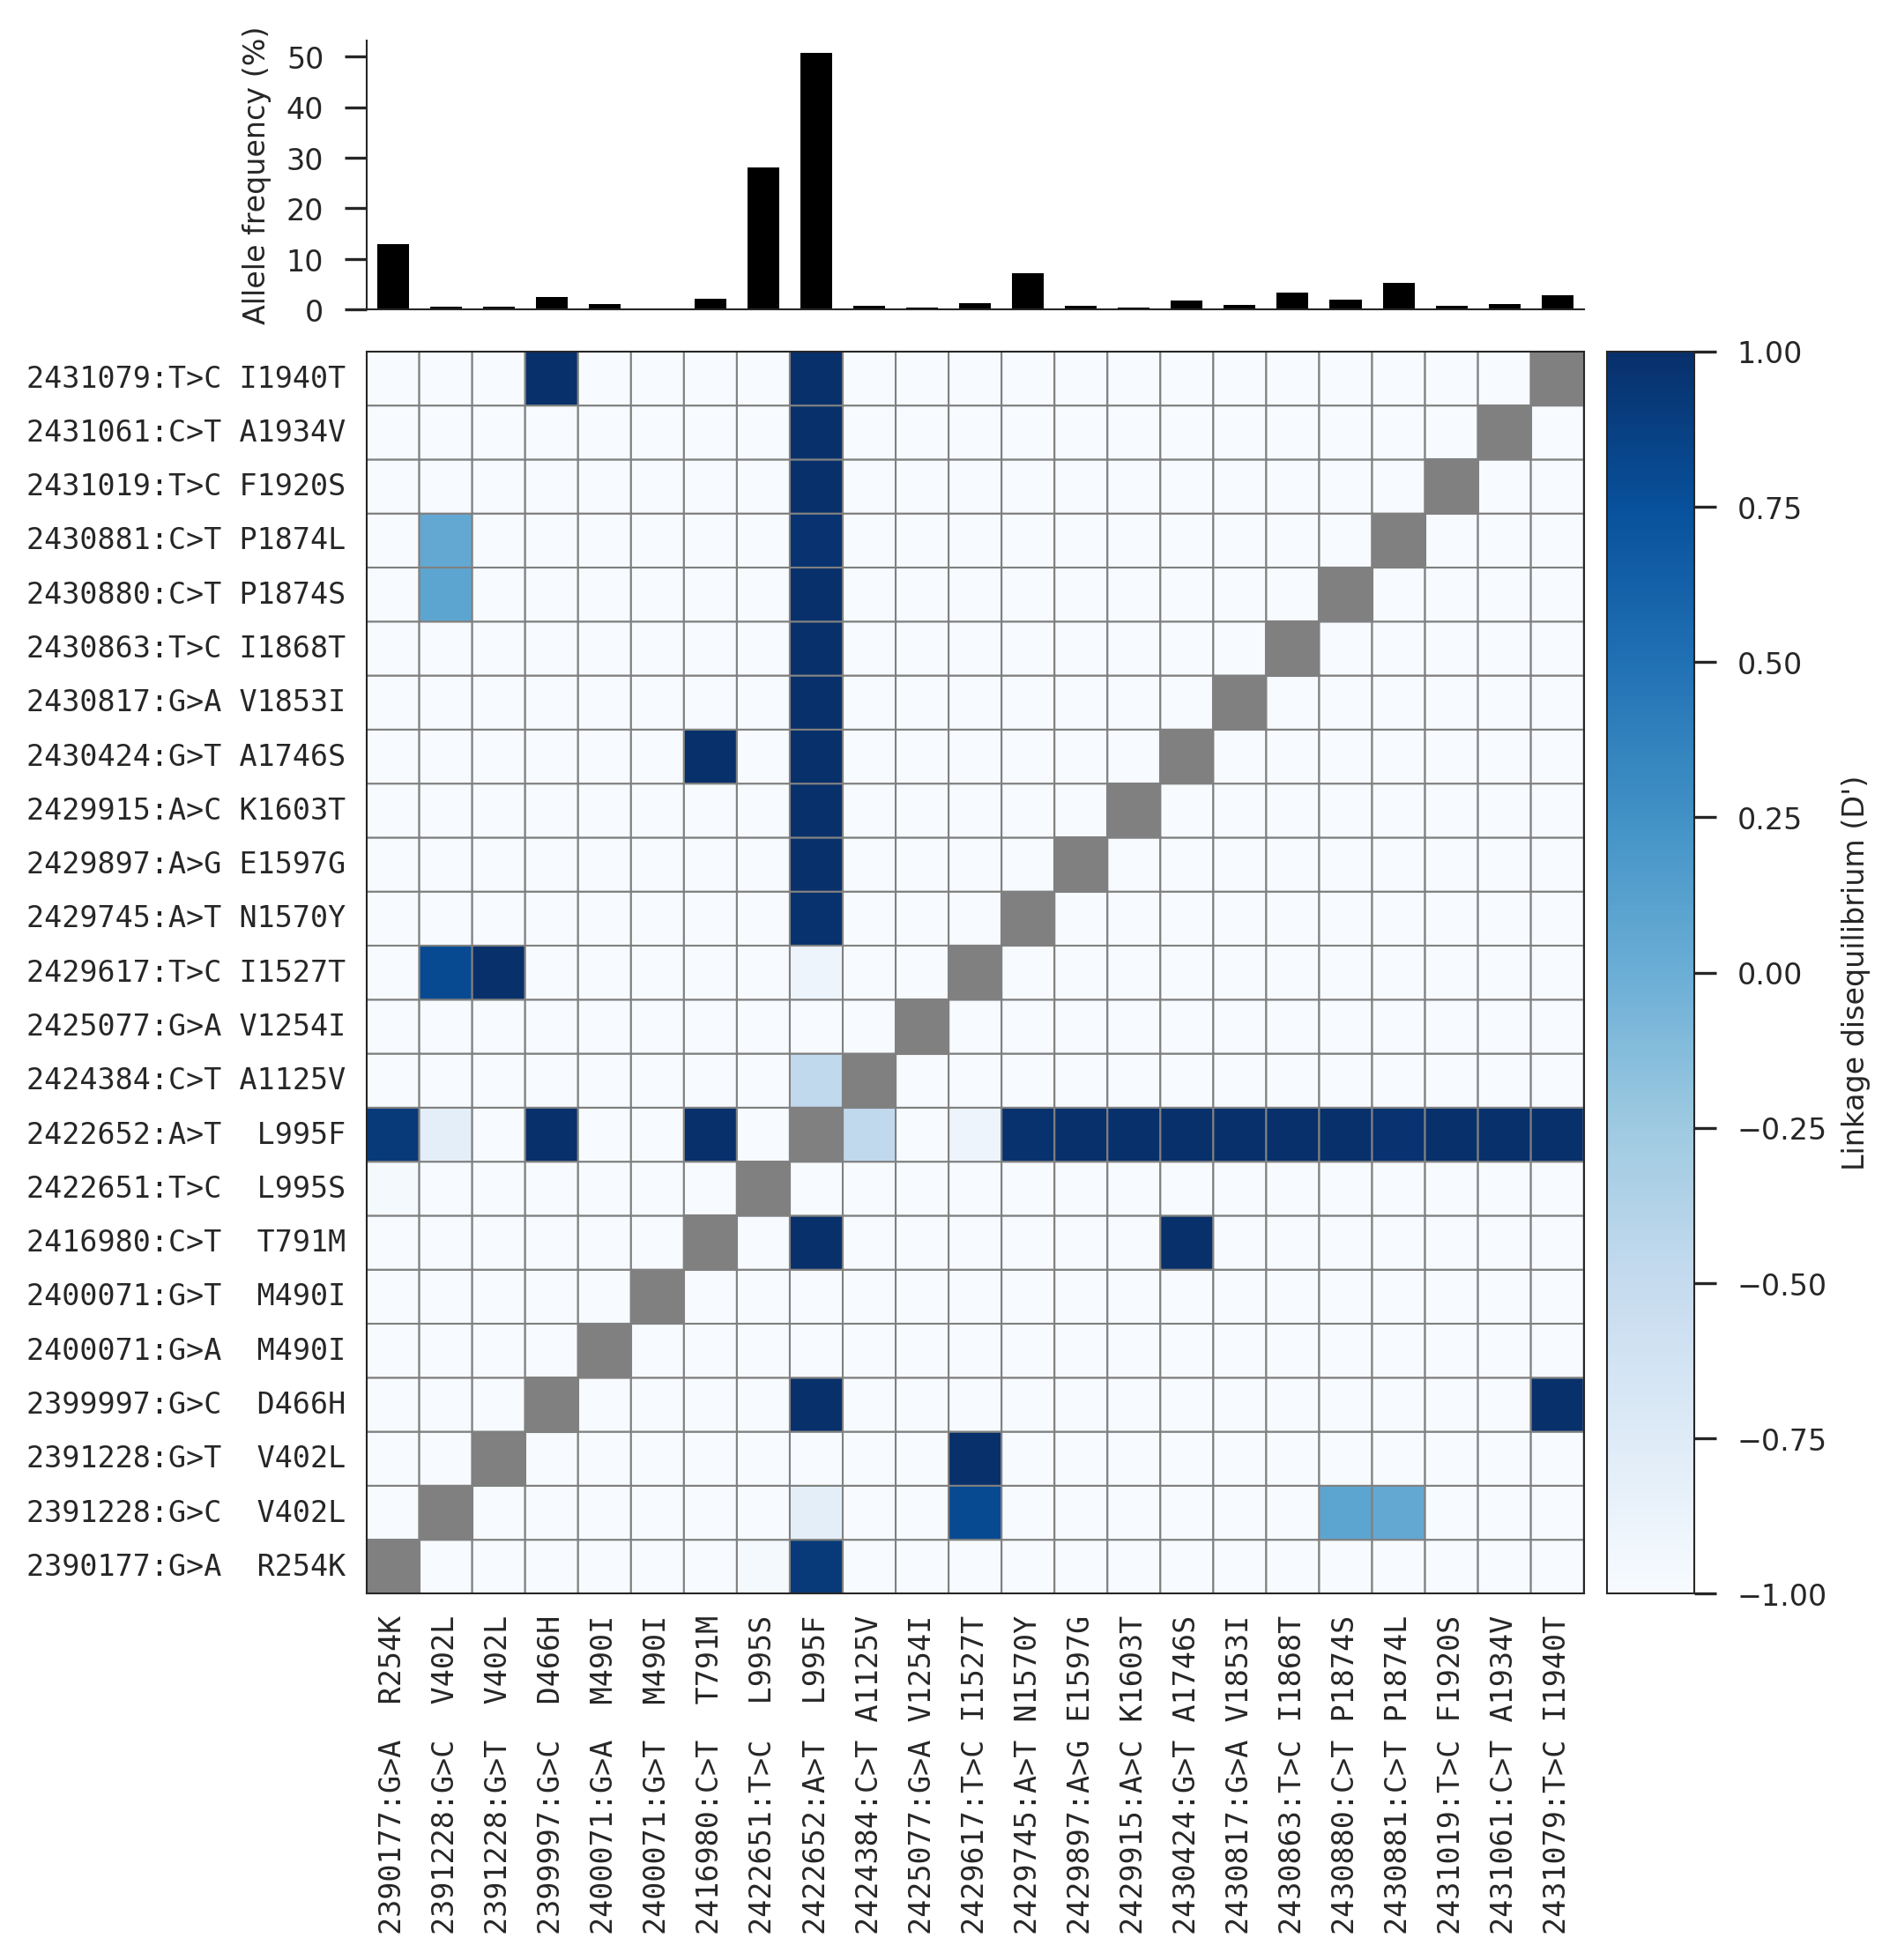
\includegraphics[width=1\linewidth,center]{artwork/fig_ld.png}
  
  \caption{\textbf{Linkage disequilibrium between non-synonymous variants}. A value of 1 indicates that the two variants always occur in combination, and conversely a value of -1 indicates that the two variants never occur in combination. @TODO nuance this?}
  
  \label{fig:ld}
\end{figure}
%%


%% Paragraph 4 - L995F enhancers.
%
Of the other 16 SNPs, 13 occurred almost exclusively in combination with \texttt{L995F} (Figure @@; @@REF Ag1000G).
%
These include the \texttt{N1570Y} allele, known to enhance pyrethroid resistance in \textit{An. gambiae} in combination with \texttt{L995F}.
%
These also include two variants in codon 1874 (\texttt{P1874S}, \texttt{P1874L}). \texttt{P1874S} has previously been found in a colony of the crop pest \textit{Plutoblah blahdiblah} with a pyrethroid resistance phenotype, but has not been shown to confer resistance experimentally.
%
10 of these variants, including \texttt{N1570Y} and \texttt{P1874S/L}, occur within internal linker domains of the protein, and so fit the model of variants that may enhance or compensate for the driver phenotype by modifying channel gating behaviour (@@CHECK; @@REFs).
%
The remaining 3 variants are within trans-membrane domains, and so may enhance resistance by @@TODO how.
%
Because of the tight linkage between these 13 SNPs and the \texttt{L995F} allele, we classify all as putative \texttt{L995F} enhancers, although experimental work is required to confirm a resistance phenotype.
%%


%% Paragraph 5 - Other high frequency variants we think are probably not resistance variants and why.
%
The remaining 3 variants (\texttt{M490I}, \texttt{A1125V}, \texttt{V1254I}) do not occur in combination with any known resistance allele, and do not appear to be associated with haplotypes under selection (@@REF Ag1000G).
%
A possible exception is the \texttt{M490I} allele found at 18\% frequency in the Kenyan population, although the fact that this population has experienced a recent population crash makes it difficult to test for evidence of selection at this locus.
%
All 3 variants occur in internal linker domains, and so do not fit the model of a resistance driver, although experimental work is required to rule out a resistance phenotype.
%
%%


%%%%%%%%%%%%%%%%%%%%%%%%%%%%%%%%%%%%%%%%%%%%%%%%%%%%%%%%%%%%%%%%%%%%%%%%%%%%%%%
\subsection*{Haplotype structure}


%
Although it is known that pyrethroid resistance is increasing in prevalence in malaria vector populations across Africa, it has not been clear whether this is being driven by the spread of resistance alleles via gene flow, or by resistance alleles emerging independently in multiple locations, or by some combination of both processes.
%
The Ag1000G data resource provides a potentially rich source of information about the evolutionary and demographic history of insecticide resistance in any given gene, because data are available not only for SNPs in gene coding regions, but also SNPs in introns and flanking intergenic regions, and in neighbouring genes.
%
These additional variants can be used to analyse the genetic backgrounds (haplotypes) on which resistance alleles are found.
%
In sexually reproducing species, DNA sequences are transmitted from parents to progeny in chunks, rearranged via recombination at each generation, and haplotypes convey information about this history of transmission and recombination, especially when haplotypes from many individuals can be compared.
%


%
In our initial analysis of the \textit{Vgsc} (@@REF Ag1000G), we used 1710 biallelic SNPs from within the @@70 kbp \textit{Vgsc} gene (@@N exonic, @@N intronic) to compute the number of SNP differences between all pairs of 1530 haplotypes derived from 765 wild-caught mosquitoes.
%
This genetic distance measurement is a rough proxy for the degree of relatedness between haplotypes, in the sense that two haplotypes with a small number of SNP differences must be closely related and share a common ancestor in the recent past.
%
This measurement cannot be used to directly estimate the time to most recent common ancestor (TMRCA) for any pair of haplotypes, however, because it does not account for the possibility of recombination events within the gene, which is increasingly likely for pairs of haplotypes that are more distantly related.
%
Nevertheless, it provides a useful tool for exploring patterns of similarity and dissimilarity within the data.
%
To visualise these patterns, we used the pairwise genetic distances to perform hierarchical clustering, which groups similar haplotypes together into clusters.
%
We found that haplotypes carrying resistance alleles were grouped into 10 distinct clusters.
%
Five of these clusters carried the \texttt{L995F} allele (labelled F1-F5), and a further five clusters carried \texttt{L995S} (labelled S1-S5).
%
Within each cluster, haplotypes were nearly identical across all 1710 SNPs (spanning @@70 kbp), and therefore each cluster represents a collection of haplotypes with a very recent common ancestor.
%
Within some of these clusters, we found haplotypes from mosquitoes collected from different locations. 
%
Specifically, cluster F1 contained haplotypes from Guinea, Burkina Faso, Cameroon and Angola; clusters @@ each contained haplotypes from Cameroon and Gabon; and cluster @@ contained haplotypes from Uganda and Kenya.
%
The F1 cluster also contained haplotypes from both \textit{An. gambiae} and \textit{An. coluzzii} individuals.
%
If we assume that haplotypes within each cluster share a common ancestor since the introduction of insecticides, which is reasonable given the high degree of similarity, then each of these clusters provides evidence that resistance alleles have been spreading between geographical locations and species via adaptive gene flow.
%
Here we present several new analyses of these haplotype data, to confirm our initial inferences regarding gene flow, and provide further details regarding the origins and movement of resistance alleles.
%


%% Figure - Haplotype networks.
%
\begin{figure}[!b]
  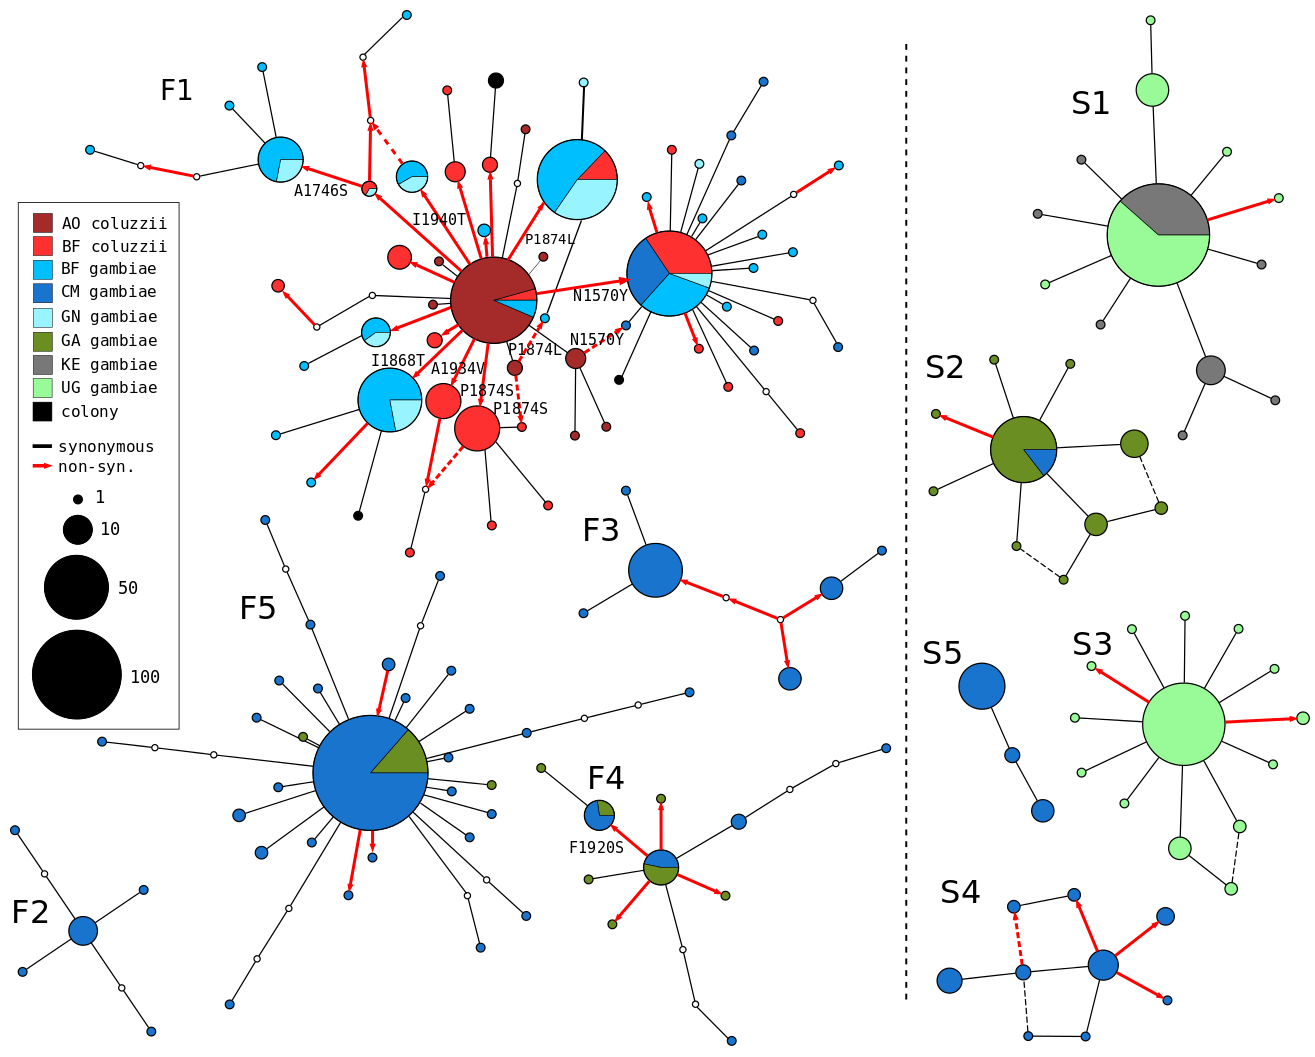
\includegraphics[width=1.1\linewidth,center]{artwork/fig_networks.png}
  \caption{\textbf{Haplotype networks}. @@TODO redo the figure. @@TODO annotate non-syn edges in cluster F3. @@TODO mention if any clusters fixed for non-syn variants so not shown. @@TODO annotate other non-syn edges, e.g., in S4?}
  \label{fig:networks}
\end{figure}
%%


%% Introduction to the networks.
%
To provide an alternative view of the genetic similarity between haplotypes carrying resistance alleles, we used haplotype data from within the Vgsc gene region to construct median-joining networks (Figure \ref{fig:networks}).
%
This analysis is very similar to hierarchical clustering, except that it allows for the reconstruction and placement of intermediate haplotypes that may not be observed in the data.
%
We constructed these networks up to a maximum distance of @@2 SNP differences, to ensure that each connected component in the resulting networks represents a collection of haplotypes with a recent common ancestor, and thus which is also likely to be minimally affected by recombination within the gene.
%
For haplotypes carrying \texttt{L995F}, the resulting network confirms the presence of five distinct clusters, with close correspondance to the clusters F1-F5 identified previously.
%
The \texttt{L995S} network also confirms five distinct clusters, in concordance with our previous analysis.
%


%% Observations from the networks.
%
The haplotype networks bring into sharp relief the explosive evolution of amino acid substitutions secondary to the \texttt{L995F} allele.
%
Within the F1 network, nodes carrying non-synonymous variants radiate out from a central node carrying only \texttt{L995F}, indicating that the central node represents the ancestral haplotype carrying \texttt{L995F} alone which initially came under selection, and these secondary variants have arisen subsequently as new mutations.
%
Many of the nodes carrying secondary variants are large, consistent with positive selection and a functional role for these secondary variants as enhancers of the \texttt{L995F} resistance phenotype.
%
The F1 network also allows us to infer multiple introgression events between the two species.
%
The central (ancestral) node comprises haplotypes from both species, as do nodes carrying the \texttt{N1570Y}, \texttt{P1874L}, and @@TODO one more variant@@.
%
This structure is consistent with an initial introgression of the ancestral F1 haplotype, followed by introgression of haplotypes carrying secondary mutations.
%
The contrast between the haplotype networks for the \texttt{L995F} and \texttt{L995S} alleles is striking because of the near-total absence of non-synonymous variation within the \texttt{L995S} networks.
%
As we reported previously, this difference is highly significant -- the ratio of non-synonymous to synonymous nucleotide diversity (@@piN/piS) is @@N times higher among haplotypes carrying \texttt{L995F} relative to haplotypes carrying \texttt{L995S} (@@Test; P=@@) (@@REF Ag1000G).
%
Some secondary variants are present within the \texttt{L995S} networks, but all are at low frequency, and thus may be neutral or mildly deleterious variants that are hitch-hiking on selective sweeps for the \texttt{L995S} allele.
%%


%% Limitations of clustering and networks based on genetic distance in a fixed region.
%
While the haplotype clustering and network analyses provide evidence for the spread of resistance alleles via adaptive gene flow, and for the secondary evolution of \texttt{L995F} enhancer alleles, they have several limitations.
%
Within haplotype clusters where gene flow has occurred, they have poor resolution to infer the origin and direction of gene flow.
%
This is because the analyses only leverage information about genetic distance within the \textit{Vgsc} gene, and for very recent events, insufficient time has elapsed for informative mutations to accumulate within this relatively small genome region.
%
Also, the fact that we observe five distinct clusters for each of the codon 995 alleles suggests that each cluster is in some sense independent from the others, and thus gene flow is not required for resistance to emerge in multiple geographical locations.
%
However, the threshold for the genetic distance at which we have chosen to divide haplotypes into different networks or clusters is to a certain extent arbitrary, and based on an intuitive sense of how much variation could have accumulated among the descendants of a single resistant ancestor since the onset of selective pressure.
%
We also need to clarify what we mean by ``independent'', as there are several possible scenarios under which resistance could evolve in multiple populations in the absence of gene flow.
%
Finally, analyses of genetic distance within a fixed genome region can be confounded by recombination events occurring within that region.
%
For example, a recombination event within the \textit{Vgsc} gene upstream of codon 995 could cause us to split a collection of haplotypes into two clusters, even though they are ancestrally related within the region downstream of the recombination event.
%
In the next sub-sections we provide some conceptual foundations to help clarify these ambiguities, and use analyses of haplotype sharing from the genome regions flanking the \textit{Vgsc} gene to provide finer resolution to diagnose recent gene flow events.
%%


%%%%%%%%%%%%%%%%%%%%%%%%%%%%%%%%%%%%%%%%%%%%%%%%%%%%%%%%%%%%%%%%%%%%%%%%%%%%%%%
\subsection*{Insecticide resistance outbreaks}


%%
%
To provide an aid to further interpretation of the genetic data, and relating them to the challenges of insecticide resistance management, we introduce the concept of an \textbf{insecticide resistance outbreak}.
%
Informally, we define a resistance outbreak by analogy with the epidemiological concept of an outbreak, as a rapid increase in the prevalence of insecticide resistance among mosquitoes at a particular place and time.
%
Note that this does not imply that the overall abundance of mosquitoes is increase, just that the relative frequency of resistance within mosquito populations is increasing.
%
We also require that all occurrences of insecticide resistance within the same outbreak are connected by a chain of transmission of resistance alleles from parent to progeny mosquitoes, and thus can be traced back to a single resistant common ancestor.
%
A resistance outbreak can be \textbf{localised}, meaning that it affects a small group of mosquitoes of a single species from a limited geographical area.
%
Alternatively, a resistance outbreak may be \textbf{spreading}, meaning that resistance alleles have been transmitted since the introduction of insecticides by interbreeding of mosquitoes of different species and/or originating from different geographical locations.
%
%%


%% Figure - Cartoon of outbreaks.
%
\begin{figure}[!b]
  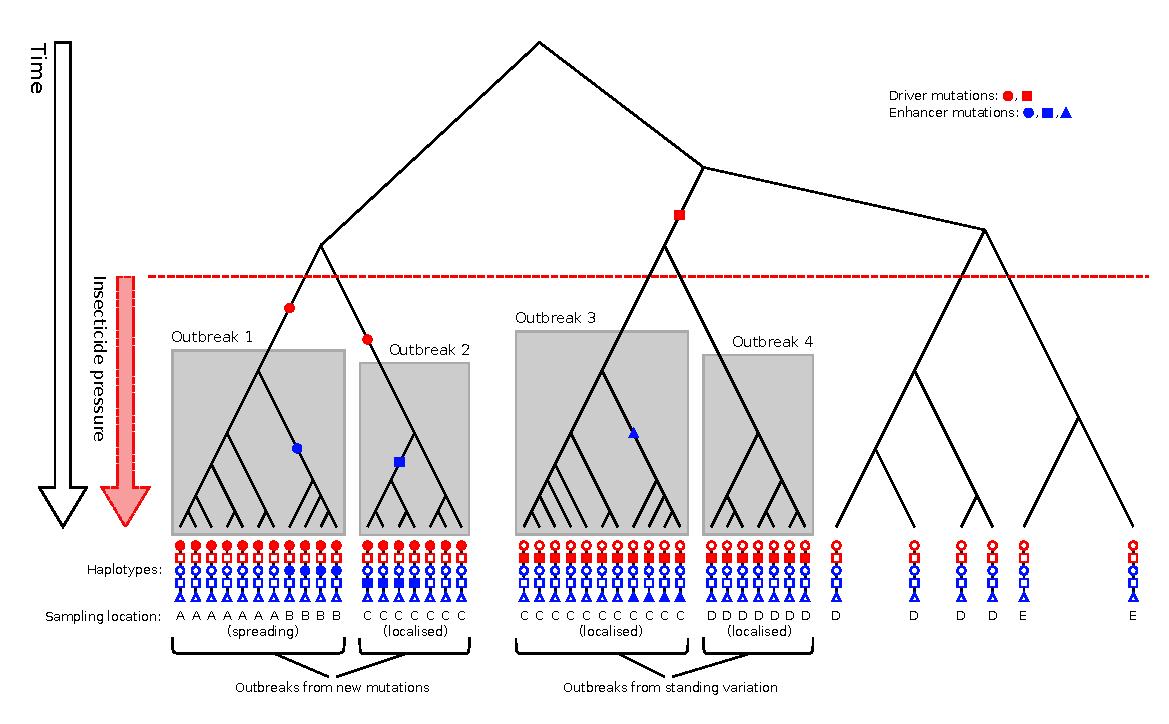
\includegraphics[width=1.1\linewidth,center]{artwork/outbreaks.pdf}
  \caption{\textbf{Illustration of insecticide resistance outbreaks}. @@TODO explanation.}
  \label{fig:outbreaks}
\end{figure}
%%


%%
%
Our goal for the \textit{Vgsc} gene can now be restated, which is to perform an insecticide resistance outbreak analysis.
%
We would like to diagnose how many separate outbreaks have occurred, which outbreaks are localised, and which are spreading.
%
For spreading outbreaks, we would like to reconstruct the path of transmission of resistance alleles between mosquito populations, and to provide information on the probable source. 
%
We would, of course, also like to identify the primary and secondary genetic factors that are driving each outbreak.
%
Stated in this way, it is easier to discuss how this information is potentially relevant to insecticide resistance management, and to frame key epidemiological questions.
%
For example, we would like to begin to build a picture of where and when local conditions have favoured the evolution of insecticide resistance, and whether those conditions are relatively patchy (and hence outbreaks are mainly localised) or whether conditions are consistent over broad areas (and hence can support a spreading outbreak).
%
We would also like to know which mosquito populations are sufficiently connected to enable outbreak spread, and if there is any consistent pattern to the direction of spread.
%
This information could be relevant to discussions about how resources for insecticide resistance management might be targeted, what strategies are appropriate in which settings, and where and when insecticide resistance management needs to be coordinated between different countries and/or at different levels of administration.
%
%%


%%
%
For clarity, we also define the concept of an insecticide resistance outbreak formally in terms of coalescent theory, as a collection of lineages (1) sharing a resistance driver allele by descent, (2) coalescing more recently than the onset of insecticide pressure, and (3) having increased in frequency because of positive selection due to insecticides. 
%
This definition is illustrated for four hypothetical outbreaks in Figure \ref{fig:outbreaks}.
%
Because mosquitoes are sexually recombining, genealogical trees vary along the genome, and so we define resistance outbreaks with respect to a specific gene locus, which for the present study is codon 995 within the \textit{Vgsc} gene.
%
Note that separate outbreaks may be driven by the same resistance allele, and this can occur if multiple mutational events occur after the introduction of insecticides (Figure \ref{fig:outbreaks}, outbreaks 1 and 2), or if a resistance allele is present in mosquito populations as standing variation prior to insecticide use (Figure \ref{fig:outbreaks}, outbreaks 3 and 4).
%
Here we are primarily concerned with whether outbreaks are localised or spreading, because this has immediate epidemiological relevance.
%
We do not attempt to infer whether separate outbreaks with the same driver allele arose via standing variation or new mutations, however this is an interesting biological question to address in future studies.
%
As a technical note, there is a simple correspondance with terminology conventionally used in the population genetics literature to describe selective sweeps.
%
At a given gene locus, a hard selective sweep gives rise to a single resistance outbreak, and a soft selective sweep gives rise to multiple resistance outbreaks.
%%


\subsection*{Outbreak analysis from haplotype age}


%% Figure - Overall haplotype age distribution.
%
\begin{figure}[!b]
  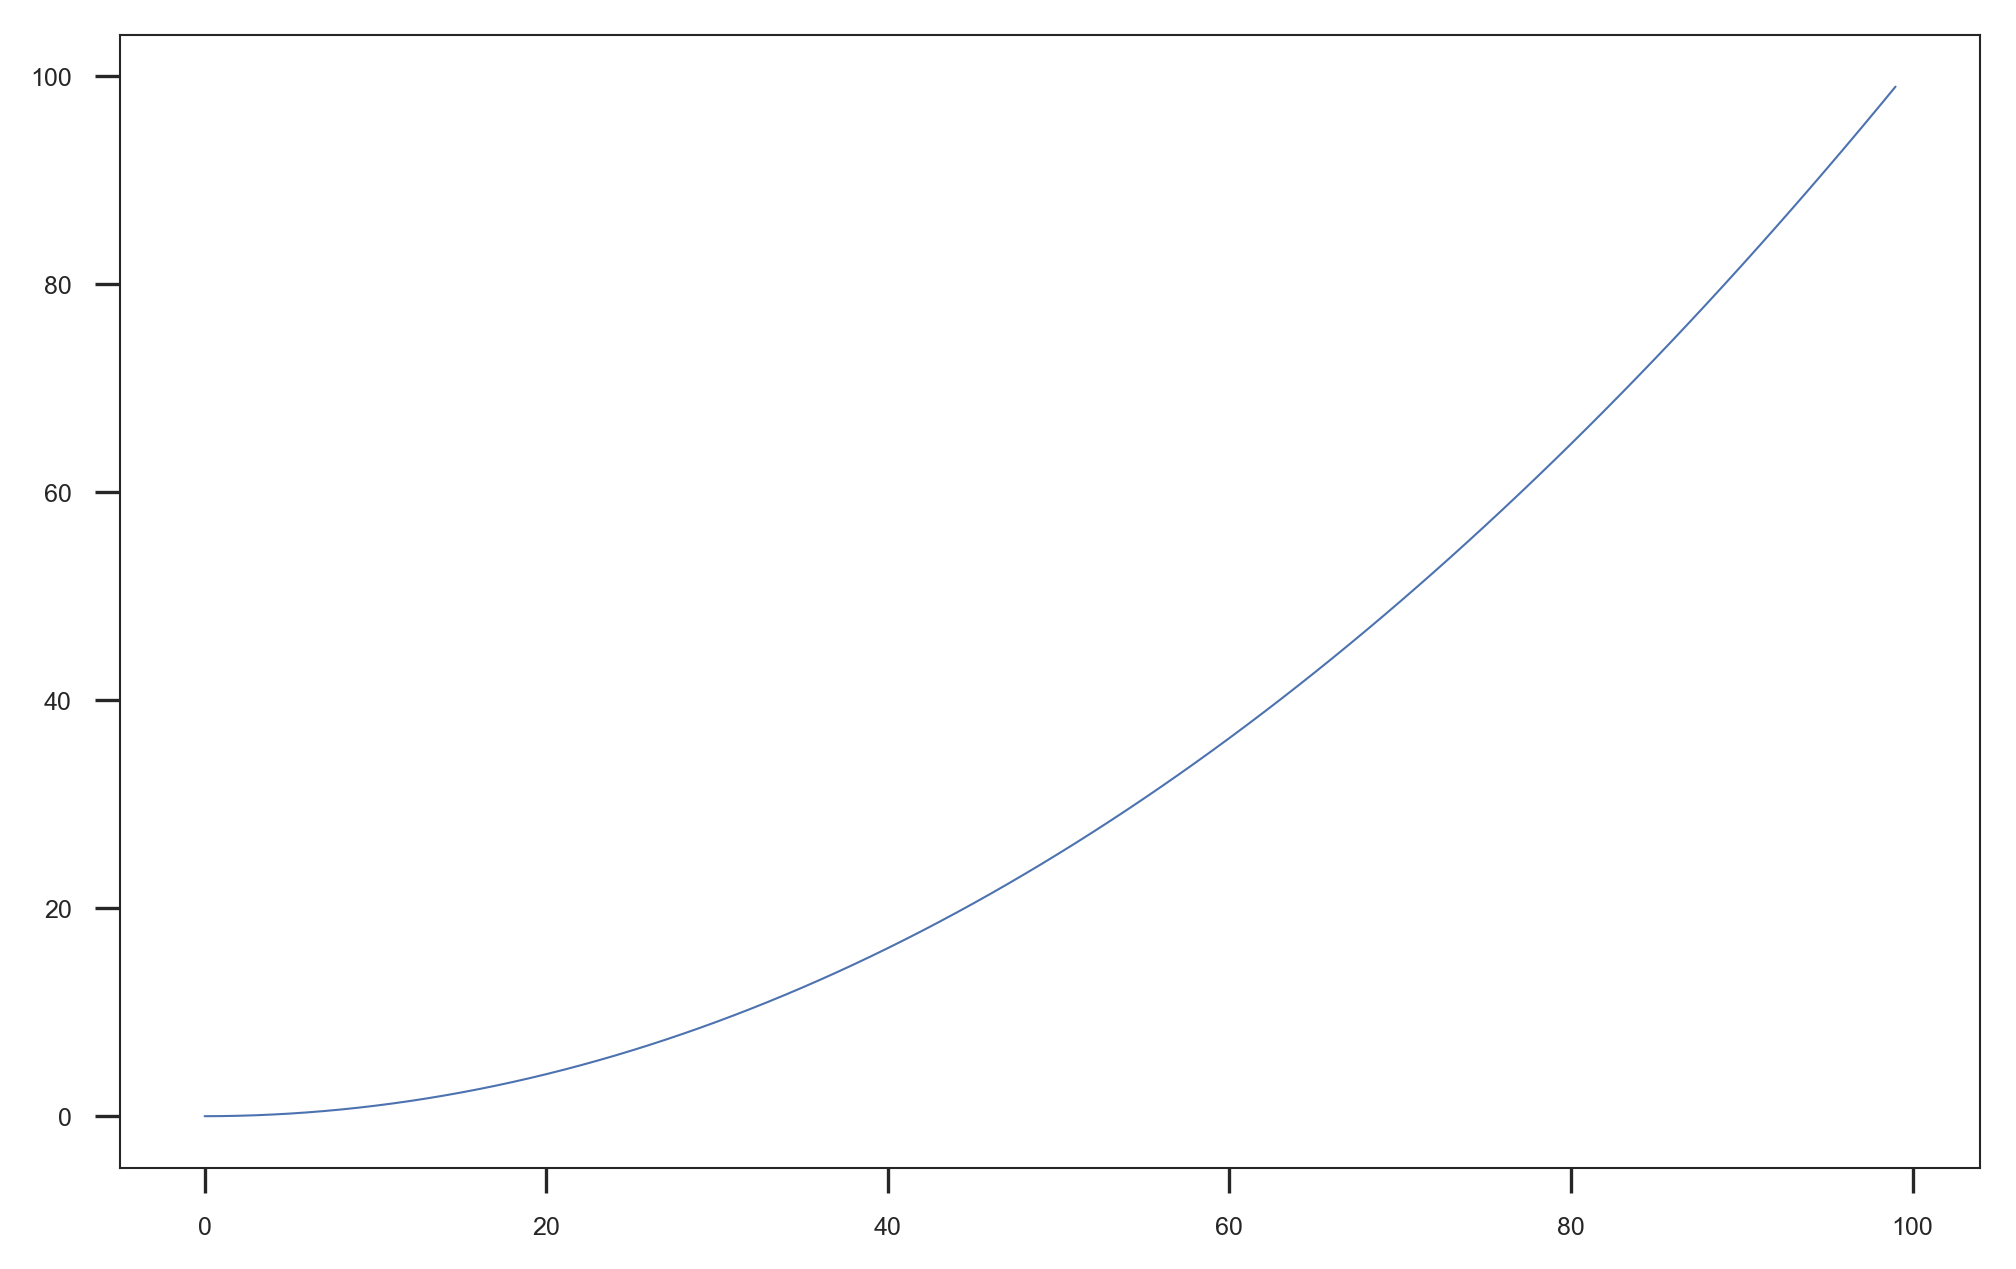
\includegraphics[width=1.1\linewidth,center]{artwork/demo.png}
  \caption{\textbf{Haplotype age distribution}. @@TODO real figure.}
  \label{fig:age_hist}
\end{figure}
%%


%%
%
As described above, haplotype data from genome regions both within and flanking the \textit{Vgsc} gene provide a higher resolution for reconstructing recent historical events.
%
To leverage this information, we used a heuristic approach to estimate the time to most recent common ancestor (TMRCA) or ``age'' for each pair of haplotypes in our dataset, centering the analysis on \textit{Vgsc} codon 995.
%
For each pair of haplotypes, we estimated the length of the region shared identical by descent (IBD), and the number of mutations that have accumulated since the most recent common ancestor.
%
We then combined these two pieces of information to produce a point estimate for the haplotype age (Methods).
%
We then studied the distribution of haplotype ages (Figure \ref{fig:age_hist}), and used hierarchical clustering to construct a dendrogram and visualise the overall age structure (Figure \ref{fig:tree}).
%
We caution that although the estimated ages are in units of generations, these estimates have not been calibrated, and there is substantial uncertainty regarding both the mutation and recombination rate parameters.
%
The ages therefore should not be interpreted as reliable absolute values, but they can be compared to each other to investigate the relative age of different events.
%%

 
%% Figure - Haplotype age tree.
%
\begin{figure}[!b]
  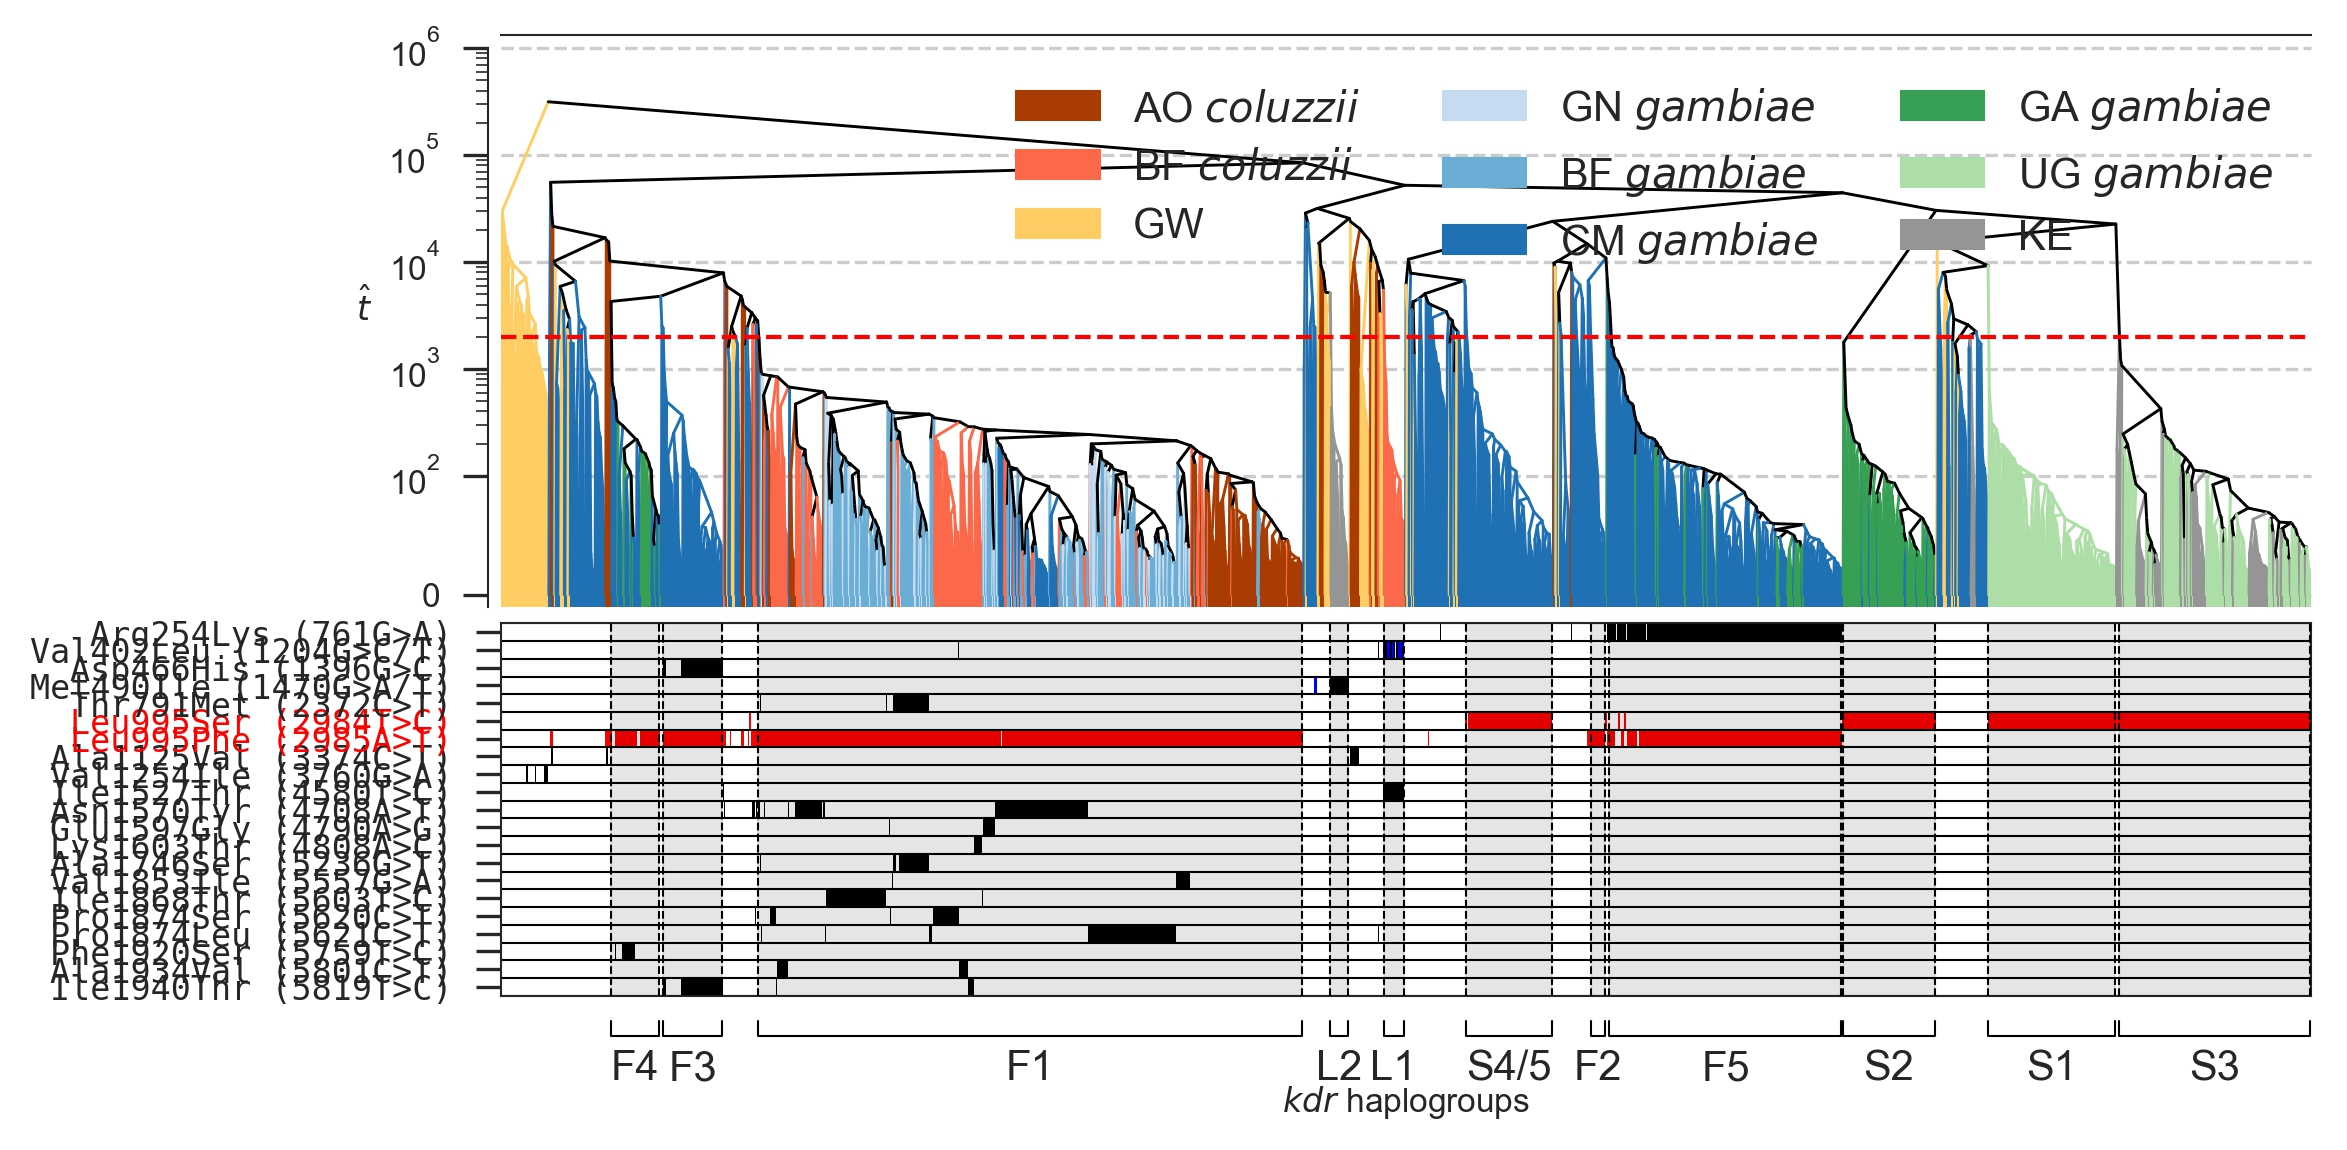
\includegraphics[width=1.1\linewidth,center]{artwork/Figure_1a_Clado.jpeg}
  \caption{\textbf{Clustering of haplotypes by age}. @@TODO bigger font. @@TODO change "kdr haplogroups" to something else. @@TODO yticks to show number of haplotypes.}
  \label{fig:tree}
\end{figure}
%%


%%
%
A key feature of the overall age distribution is that it is bimodal, with a minor mode of haplotypes coalescing recently, and a major mode coalescing further in the past (Figure \ref{fig:age_hist}).
%
This is expected at an insecticide resistance locus experiencing one or more resistance outbreaks.
%
Within each outbreak, all haplotypes share a very recent common ancestor, but between outbreaks and among haplotypes without any resistance allele, haplotypes are more distantly related, and the distribution of ages is influenced by mosquito population size and other demographic factors.
%
The bimodal age distribution is not due to geographical population structure, because the same bimodality is observed within several populations.
%
We take the midpoint between these two modes as an estimate for the earliest time of onset of selective pressure due to insecticides, and thus for the maximum age of a resistance outbreak.
%
To identify haplotype clusters representing putative resistance outbreaks, we then cut the haplotype dendrogram at this maximum outbreak age (Figure \ref{fig:tree}).
%
Comparing this to previous analyses of haplotype structure based on genetic distance, we find clusters F1-F5 and S1-S3 recapitulated with close correspondence, and S4 and S5 merged into a single cluster.
%
We label a new cluster ``L@@'' representing an outbreak driven by the \texttt{I1527T} allele in combination with one or the other \texttt{V402L} allele.
%
We also label a cluster ``L@@'' capturing a set of haplotypes from Kenya carrying the \texttt{M490I} variant, although the fact that these haplotypes all share a recent common ancestor may be a reflection of the extreme demography of the Kenyan population (@@REF) and not reflect recent selection for insecticide resistance.
%
As in earlier analyses, clusters F1, F4, F5 and S3 all include haplotypes sampled from multiple geographical locations, and thus represent spreading outbreaks.
%
Clusters F2, F3, S1, S2, S4/5 and L1 include only haplotypes from a single sampling location, and thus appear to represent localised outbreaks.
%%


%% Figure - Infering spread
%
\begin{figure}[!b]
  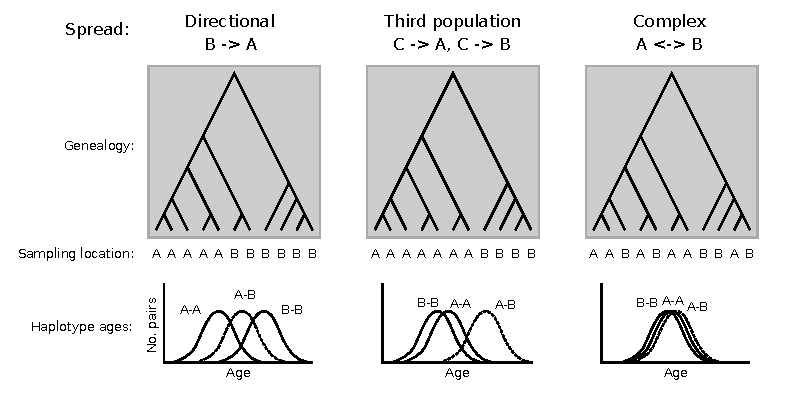
\includegraphics[width=1.1\linewidth,center]{artwork/spreading.pdf}
  \caption{\textbf{Inferring history of spread from haplotype ages}. @@TODO explain.}
  \label{fig:spreading_cartoon}
\end{figure}
%%


%%
%
We then studied the distribution of haplotype ages within each spreading outbreak, to attempt to reconstruct information about the historical path of transmission of resistance alleles between locations.
%
To do this, we decompose each spreading outbreak into separate sampling locations, and compared the distribution of haplotype ages both within and between locations.
%
We define three possible spreading scenarios, being: (1) a directional spread from one population to another; (2) spread from an unsampled population into the sampled populations; and (3) a complex scenario involving multiple gene flow events.
%
In Figure \ref{fig:spreading_cartoon} we illustrate the expected genealogy and haplotype age distribution under each of these scenarios.
%
The clearest result is obtained for outbreak F1 (Figure \ref{fig:outbreak_spread}).
%
Within this outbreak, haplotypes from Cameroon and Angola are younger than haplotypes from Burkina Faso and Guinea.
%
The age distributions are consistent with an outbreak originating in West Africa and subsequently spreading towards Cameroon and separately towards Angola.
%
Interestingly the age distributions for \textit{An. gambiae} and \textit{An. coluzzii} from Burkina Faso are very similar, despite the fact that previous studies have shown the direction of introgression has occurred from \textit{An. gambiae} into \textit{An. coluzzii}.
%
This may indicate that introgression happened during the early phases of the outbreak, but is also consistent with a complex history of multiple gene flow events between the species.
%%


%% Figure - Age distributions within haplogroups. Include results for Cameroon/Gabon haplogroups.
%
\begin{figure}[!b]
  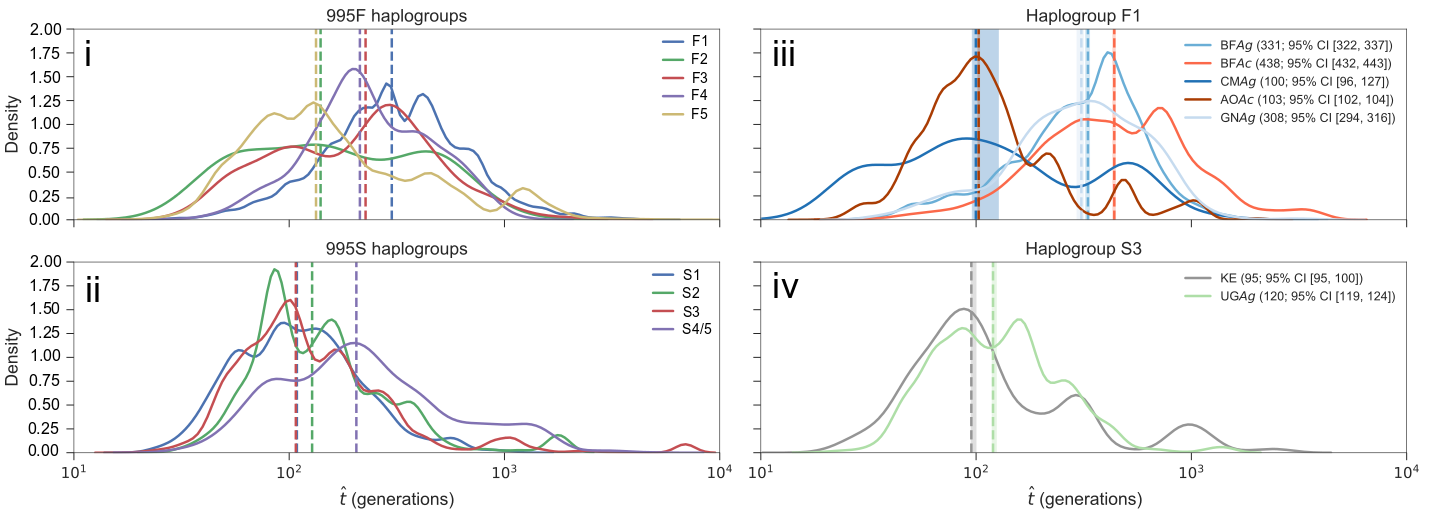
\includegraphics[width=1.1\linewidth,center]{artwork/Figure_3_RelativeAges_tweak_final.png}
  \caption{\textbf{Haplotype age distributions}. @@TODO rethink what goes in here, also if this needs to be here or can go to supplementary.}
  \label{fig:outbreak_spread}
\end{figure}
%%





@@TODO



%%%%%%%%%%%%%%%%%%%%%%%%%%%%%%%%%%%%%%%%%%%%%%%%%%%%%%%%%%%%%%%%%%%%%%%%%%%%%%%
%%%%%%%%%%%%%%%%%%%%%%%%%%%%%%%%%%%%%%%%%%%%%%%%%%%%%%%%%%%%%%%%%%%%%%%%%%%%%%%
\section*{Discussion}


@@TODO Discuss accessibility, have we missed any functional variation?


@@TODO Discuss weaknesses, caveats and potential improvements to method for estimating haplotype age.


@@TODO What are the implications for insecticide resistance management? Realistically how could this information be used?


@@TODO What about DDT? If prior selection for DDT resistance, how might this complicate the picture? Do we see any evidence for multiple phases of selection?


@@TODO Speculate on why \texttt{L995F} but not \texttt{L995S} has evolved secondary variation.



%%%%%%%%%%%%%%%%%%%%%%%%%%%%%%%%%%%%%%%%%%%%%%%%%%%%%%%%%%%%%%%%%%%%%%%%%%%%%%%
\section*{Legacy}





%% Paragraph 7? - Bringing results together, display on map...
%
@@TODO describe how we put together the map (Figure \ref{fig:map}).
%%


%% Figure - Map of haplotypes and spread.
%
\begin{figure}[!b]
  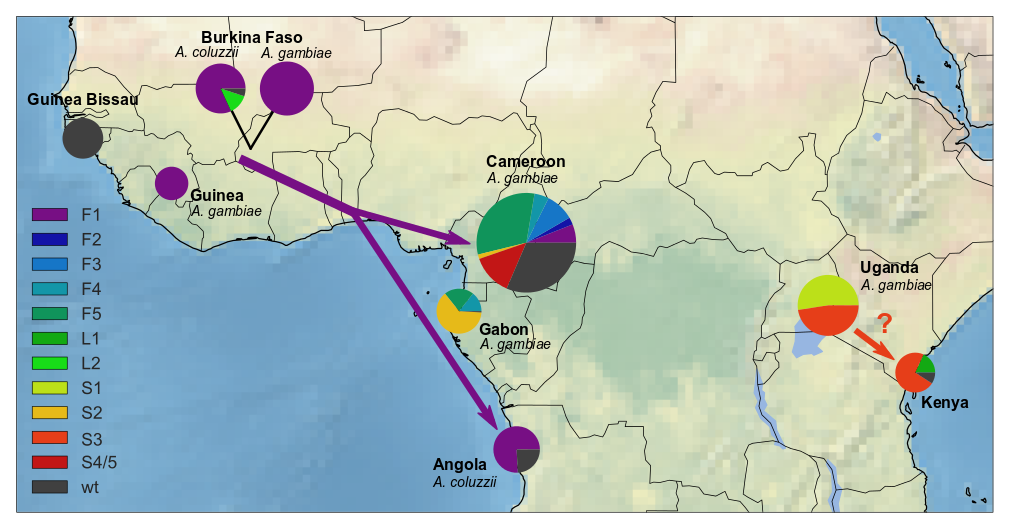
\includegraphics[width=1.1\linewidth,center]{artwork/fig_map.png}
  \caption{\textbf{Geographical distribution of resistance haplogroups}. }
  \label{fig:map}
\end{figure}
%%


\subsection*{Recombination and independent outbreaks of resistance}


%% Paragraph 1 - Introduce the problem/question, what do we want to infer? We want to infer independent outbreaks of resistance, a.k.a., multiple local origins/outbreaks, by which we mean ... @@TODO. haplotype clusters appear distinct but recombination events could occur during geographical spread, bringing resistance onto a different genetic backgrounds.
%
@@TODO
%%


%% Paragraph 2 - Say what analysis we did to address this - which is, reconstruct putative ancestral haplotype for each haplogroup. Then scan all haplotypes against, computing distinct (divergence) in windows (Figure 7; Figure 8).
%
@@TODO
%%


%% Figure - L995F recombination
%
\begin{figure}[!b]
  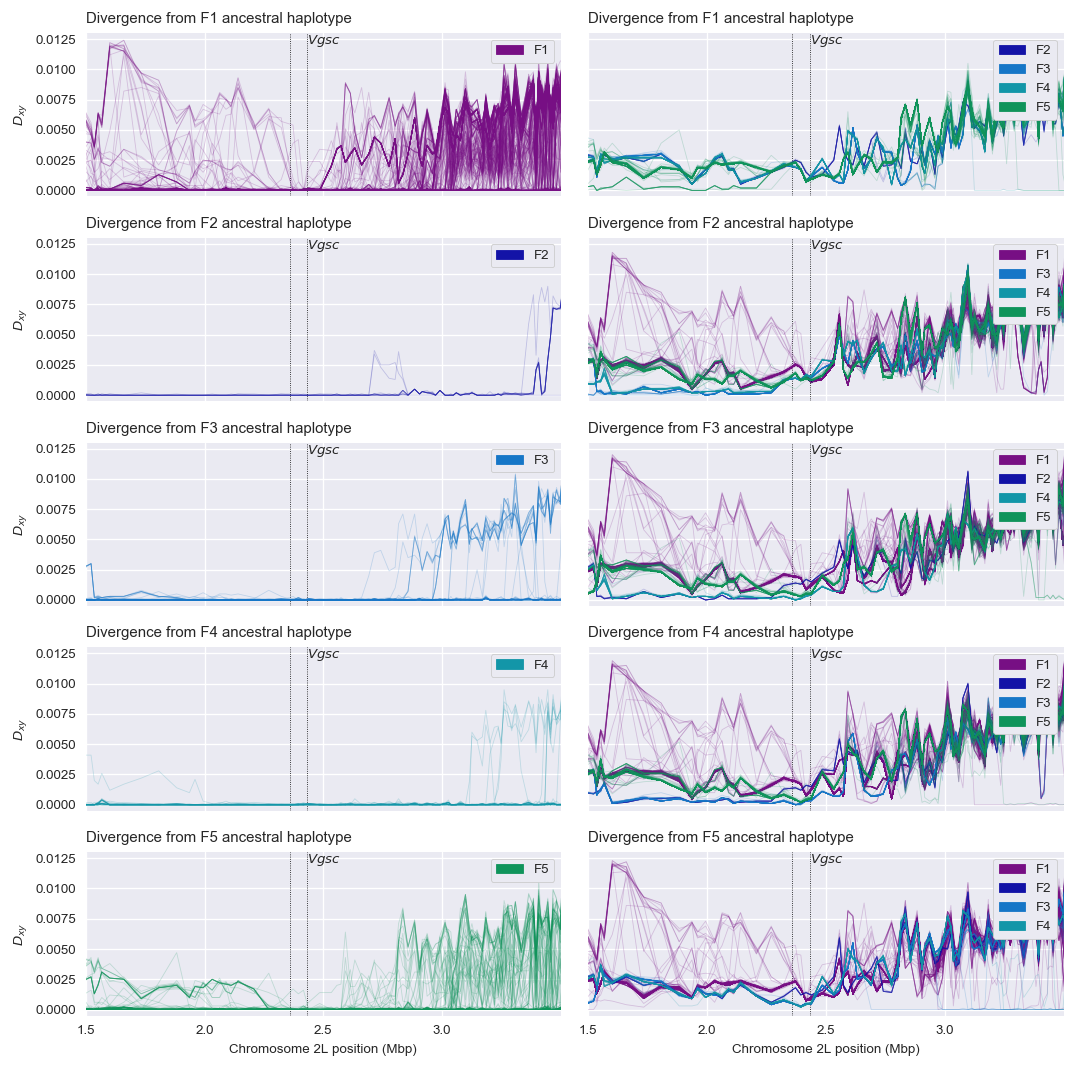
\includegraphics[width=1.1\linewidth,center]{artwork/fig_recom.png}
  \caption{\textbf{Recombination and ancestral haplotypes for L995F}. @@TODO legend}
  \label{fig:recom_f}
\end{figure}
%%


%% Paragraph 3 - Describe results of scans, evidence for independent outbreaks.
%
@@TODO
%%


%% Figure - L995S recombination
%
\begin{figure}[!b]
  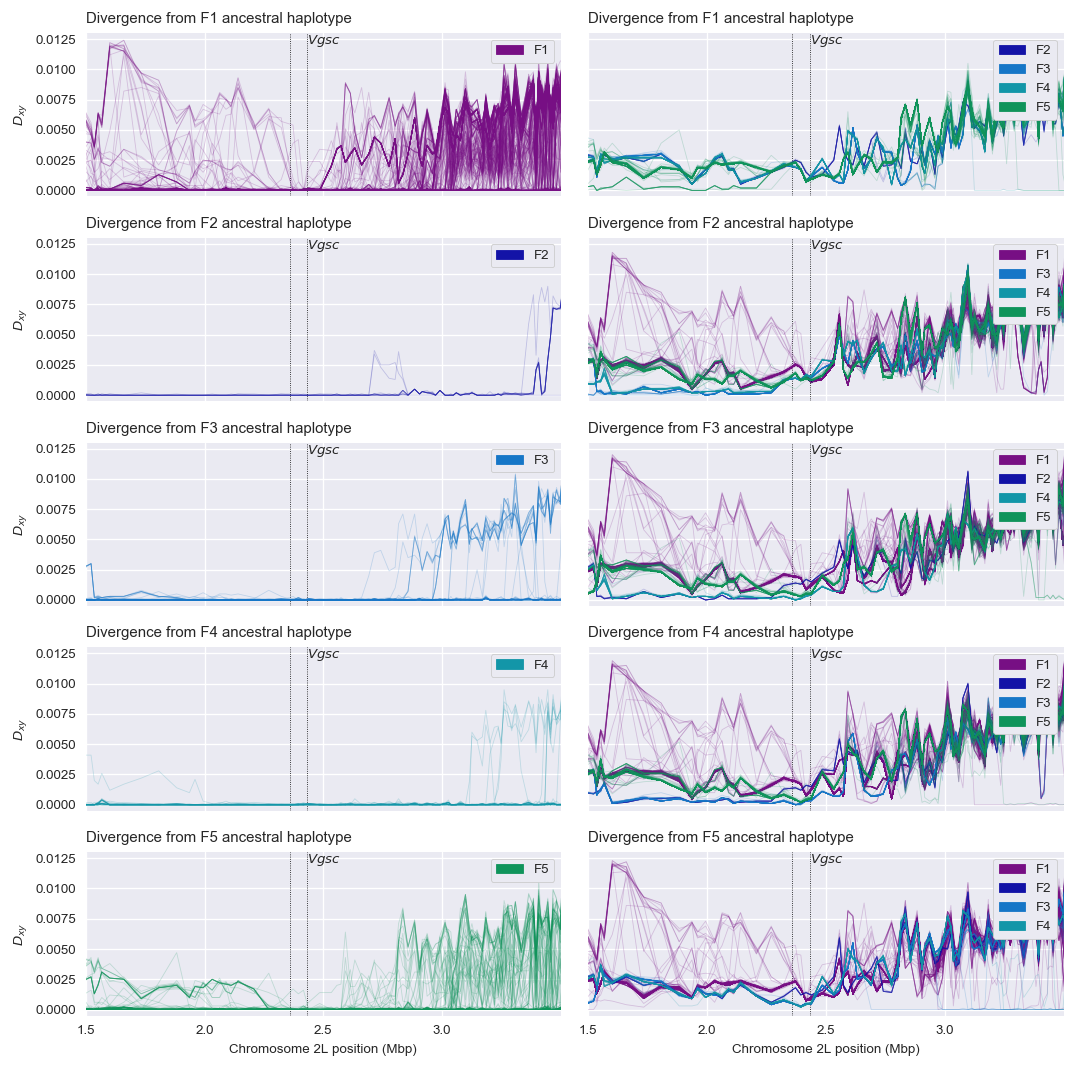
\includegraphics[width=1.1\linewidth,center]{artwork/fig_recom.png}
  \caption{\textbf{Recombination and ancestral haplotypes for L995S}. @@TODO legend}
  \label{fig:recom_s}
\end{figure}
%%


\section*{Discussion}

@@TODO


\section*{Methods}

@@TODO

\printbibliography

\end{document}
